\documentclass[border=2pt]{standalone}
\usepackage[dvipsnames,svgnames,x11names]{xcolor}
\usepackage{tikz}
\usepackage{pgfplots}
\usetikzlibrary{calc,arrows.meta,positioning,intersections}
\usepgfplotslibrary{fillbetween}
\pgfplotsset{compat=1.18}

\pgfplotsset{
  funfig axis/.style={
    width=10cm,
    height=7cm,
    grid=major,
    grid style={draw=gray!25,line width=0.2pt},
    axis line style={line width=0.5pt},
    tick style={line width=0.45pt},
    legend style={draw=none,fill=none,cells={anchor=west}},
  },
}

\begin{document}
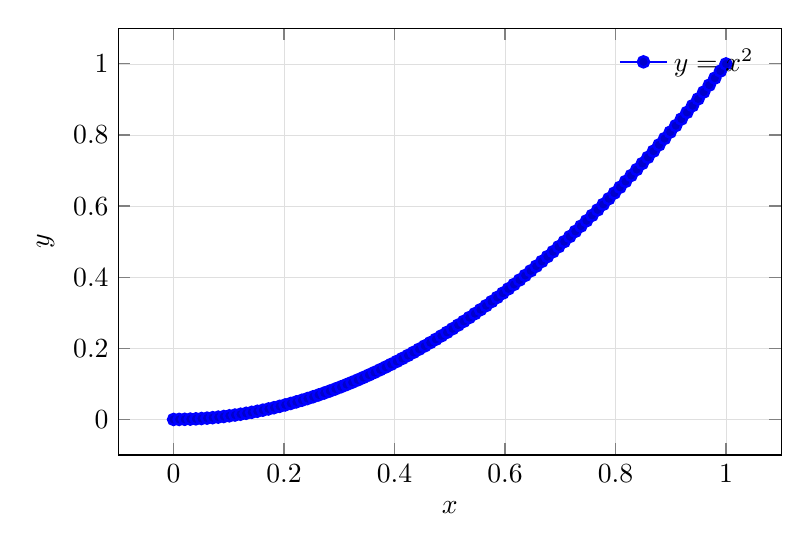
\begin{tikzpicture}
  \begin{axis}[
    funfig axis,
    xlabel={$x$},
    ylabel={$y$},
  ]
    \addplot+[domain=0:1,samples=100,line width=0.9pt] {x^2};
    \addlegendentry{$y=x^2$}
  \end{axis}
\end{tikzpicture}
\end{document}

